\chapter{Model}
\label{chapter4}
\section{Arcachon basin}
To do the simulation it is necessary to choose a location that has a lot of data available and a favorable geography, so we chose the Arcachon basin to do our simulation. The figure below shows the topology and bathymetry of this region.
The dataset was obtained from Shom France and OpenTopoData.
\vspace*{-0.85cm}
\begin{figure}[h]
    \hspace*{-1.5cm}
    \begin{subfigure}{0.5\textwidth}
        \centering
        \includegraphics[scale=0.5]{images/Mesh/Mar_data.png}
        \caption{Bathymetry}
        \label{fig:sub1}
    \end{subfigure}%
    \hspace*{-2.7cm}
    \begin{subfigure}{0.5\textwidth}
        \centering
        \includegraphics[scale=0.5]{images/Mesh/Topo_data.png}
        \caption{Topography}
        \label{fig:sub2}
    \end{subfigure}%
    \hspace*{-2.7cm}
    \begin{subfigure}{0.5\textwidth}
        \centering
        \includegraphics[scale=0.5]{images/Mesh/Topo_Mar_data.png}
        \caption{Topography and bathymetry}
        \label{fig:sub3}
    \end{subfigure}%
    \caption{Real datas for topography and bathymetry, on scale is the depth in meters}
    \label{fig:test}
    \end{figure}

\vspace{-0.75cm}
\section{Our approach}
With the data obtained from the topology and topography of this region, the delaunay method from the PyVista library was used to make the mesh. However, due to the way the data is collected in real life, there are very sharp variations in the height of the relief.
Thus, it is necessary to smooth these aspects, for this, we used the k-nearest neighbors (k-NN) with k=7 to make a mean and update the depth for each element in order to obtain a more regular structure. The figure below shows the mesh obtained for the dataset mentioned before.
\begin{figure}[h]
\begin{subfigure}{.5\textwidth}
    \centering
    \includegraphics[width=0.7\linewidth]{images/Mesh/mesh_wireframe1.png}
    \caption{Topography and bathymetry}
    \label{fig:sub1}
\end{subfigure}%
\begin{subfigure}{0.6\textwidth}
    \centering
    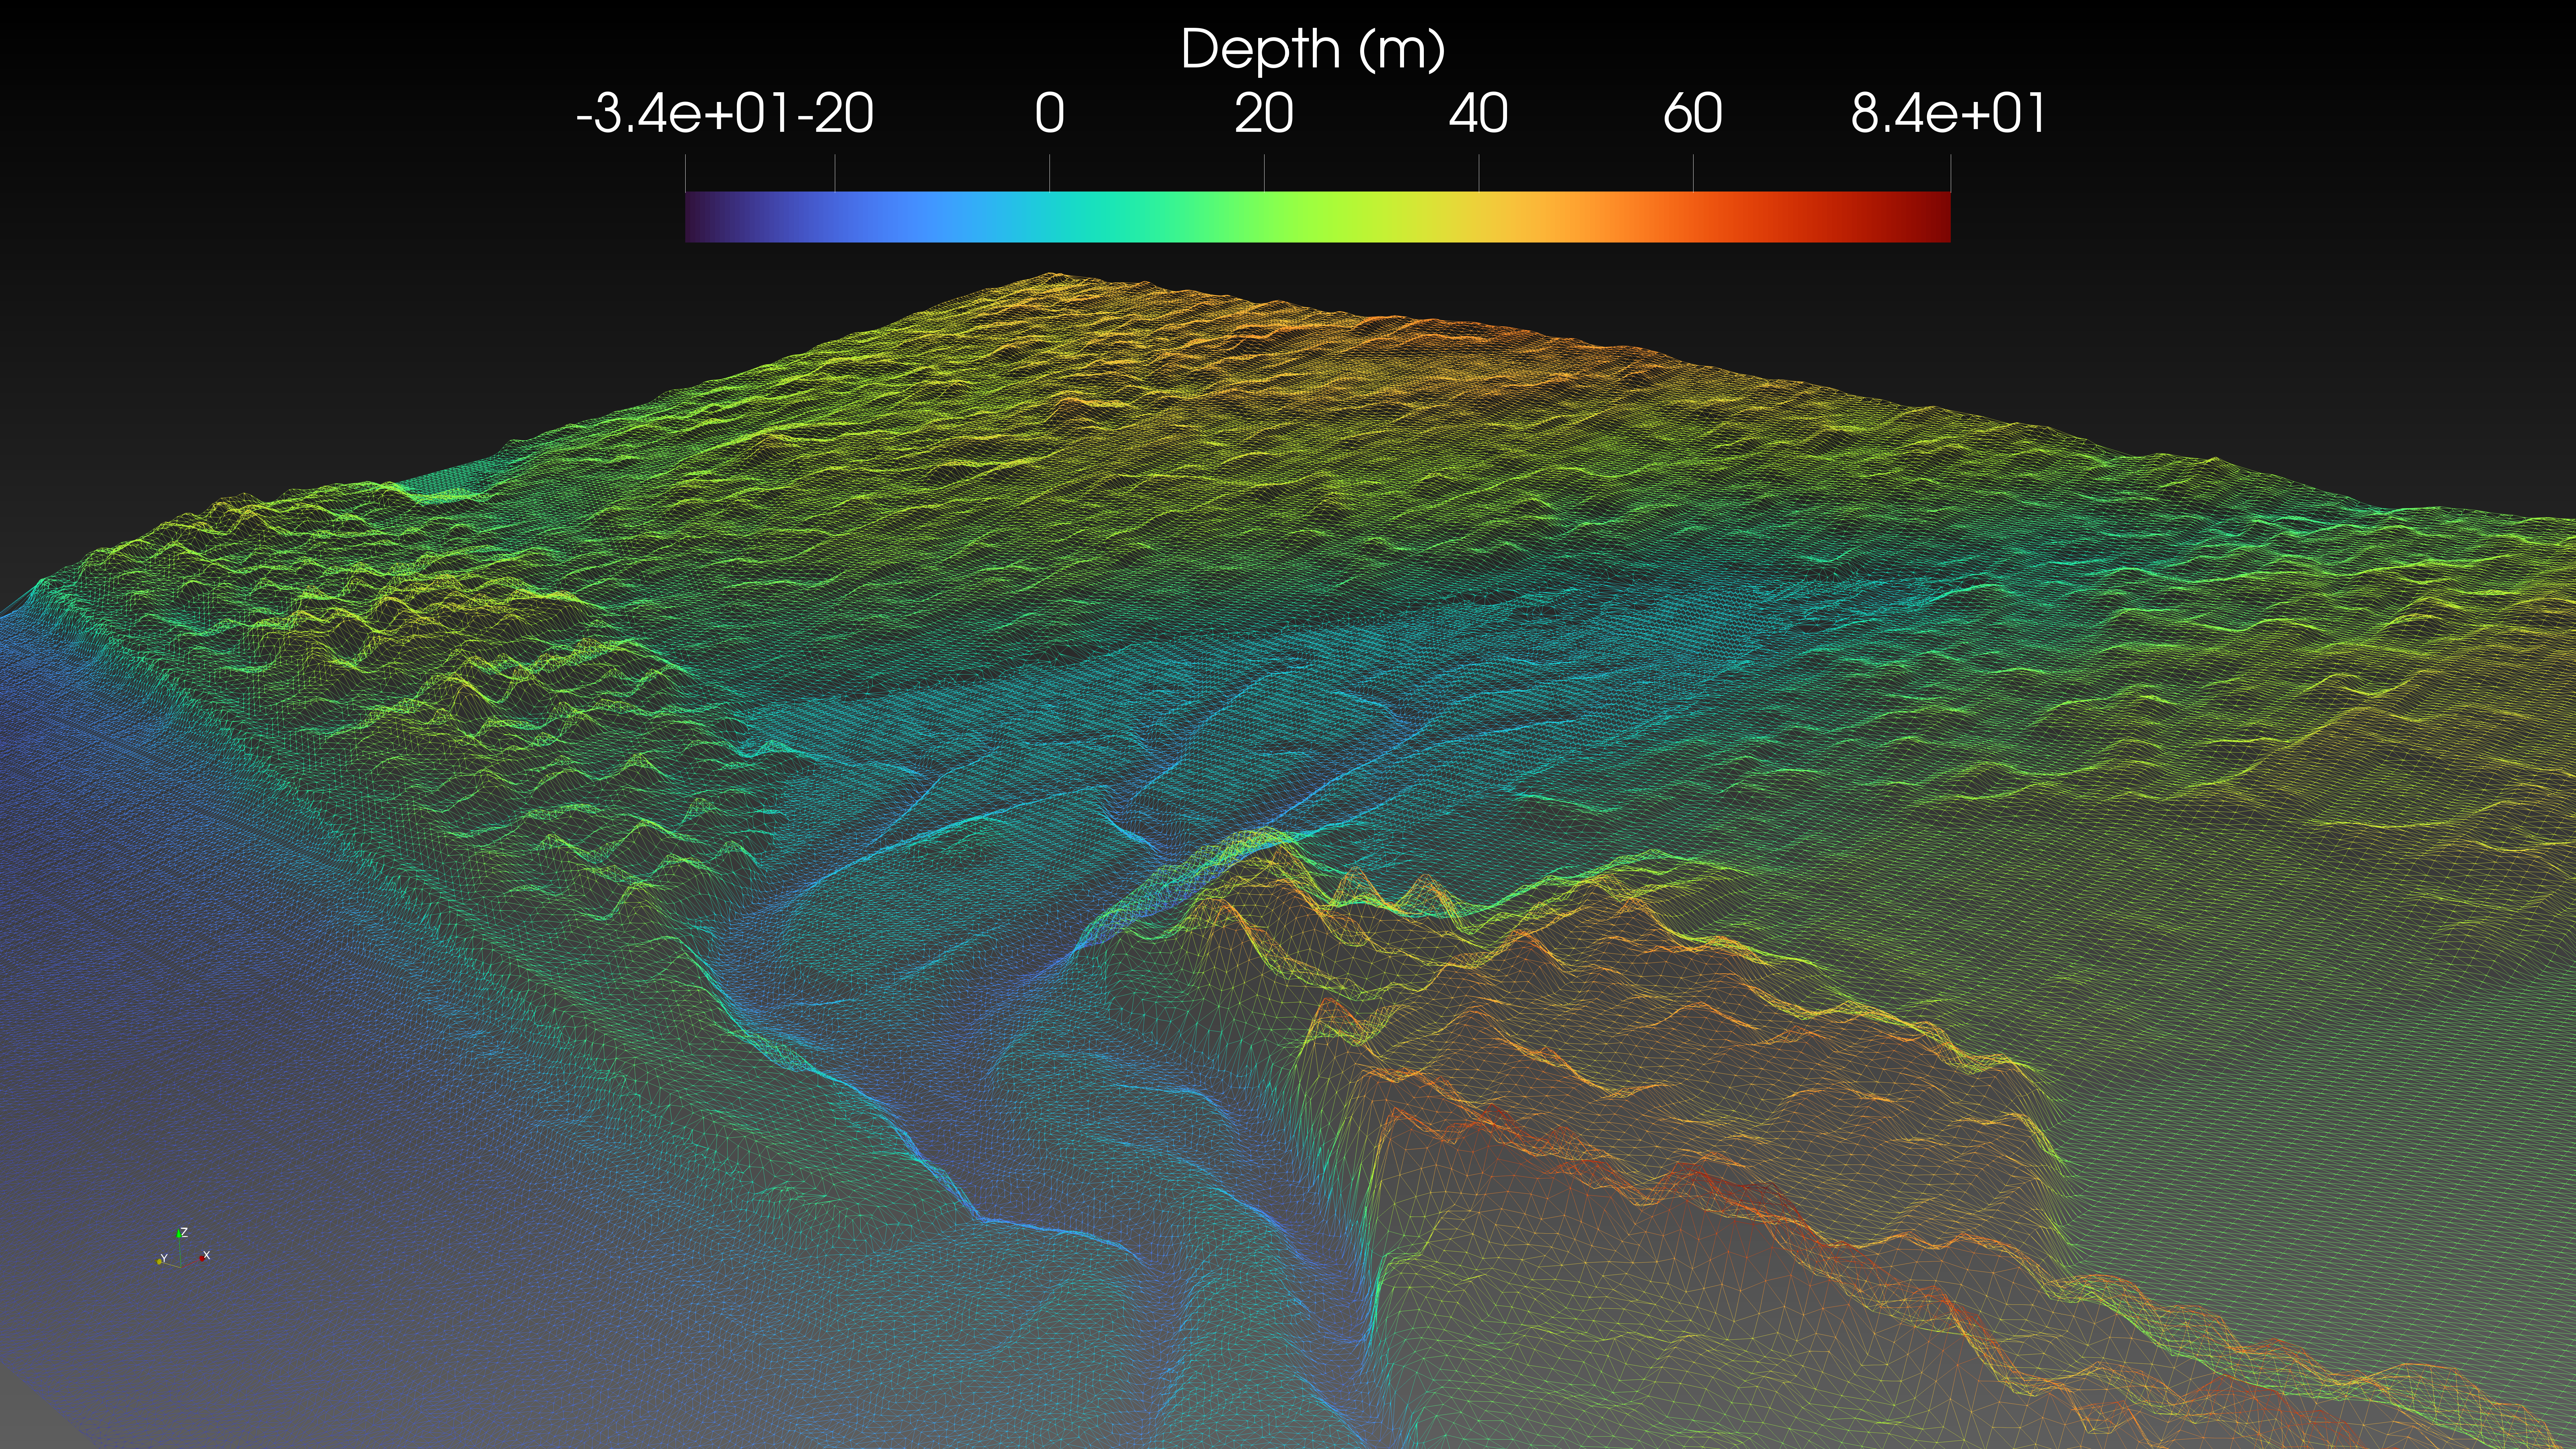
\includegraphics[width=0.8\linewidth]{images/Mesh/mesh_wireframe.png}
    \caption{Wireframe}
    \label{fig:sub2}
\end{subfigure}%
\caption{Arcachon basin mesh}
\label{fig:test}
\end{figure}

\vspace{-0.75cm}
\section{Parallel processing}
The obtained structure has about 280000 elements and according to the simulations performed on chapter \ref{chapter3}, a very high number of loops will be required for the neural network to provide a good solution. However, due to the dimensions of the Mesh, the computational cost is very high, so a different approach is needed to do the simulation.
A very effective way to do this is to use parallel computing, i.e. the domain is divided into several subdomains that will be processed in different cores so that the same task is divided into small subtasks to speed up the final operation. 
So at each step of the main loop the neural net is put to train in the sub-domains, and then at the end of each loop the performance of the net is evaluated.
This procedure is described in the pseudo-code below.
\begin{algorithm}[H]
    \caption*{Gradient descent with parallel computing}
    \hspace*{\algorithmicindent} \textbf{Input}  NN\_parametres, p the number of simultaneous subtasks, loss\_function\\
    \hspace*{\algorithmicindent} \textbf{Output} new parametres
    \begin{algorithmic}
    \STATE repeat until convergence
        \bindent 
        \STATE get a training set and divide it into p-subsets with the same number of elements 
        \FOR {each n-processor}
            \STATE evaluate loss\_function of the n-subset
        \ENDFOR
        \STATE concatenate the p-set values obtained in the same training set order
        \STATE make gradient descent and update the parametres  
        \eindent
    \end{algorithmic}
    \end{algorithm}
    
\begin{itemize}
    \item To do this in Python we can use vmap function of Jax library to vectorize the gradient descent
\end{itemize}

\section{Mild slope equation}